When discussing trajectory generation, we previously overlooked the dimension of time. For a robot, it is not only important to consider the constraints imposed by obstacles but also the robot itself. Robots often have inherent limitations, such as constraints on their velocities and accelerations, which must be accounted for at every point along the trajectory. To address this, we now present several methods capable of generating an initial trajectory and optimizing it to satisfy these constraints. We can formalize the problem as an optimization problem, as defined in \ref{eq:optimization_problem}, with constraints related to the system dynamics and the initial path.

AS we can see this stage is an important one, since the trajectory generated but an algorithm such as RRT that does not take into consideration the dynamics of the system may generate an infeasible path, as shown in Figure~\ref{eq:Proposed Approach: Space Cobot: Bad trajectory generation}, where the rough path for the robot would lead to an unfeasible configuration, and so the optimized path needed to first go backwards.

\begin{figure}
    \centering
    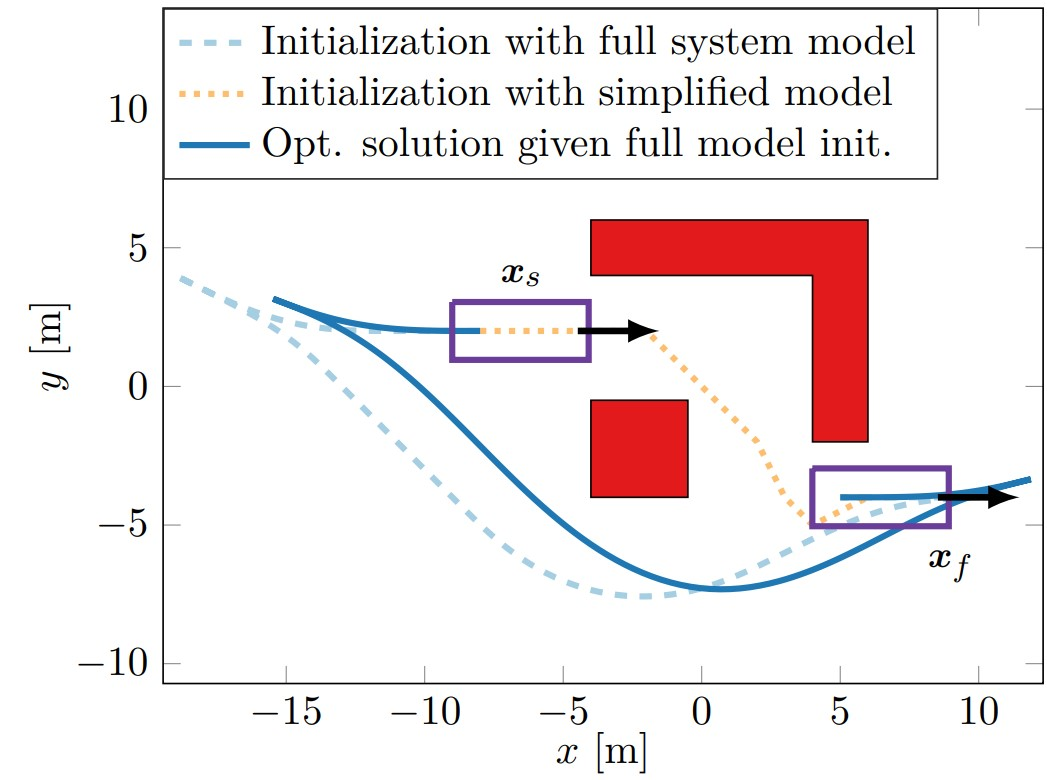
\includegraphics[width=0.7\textwidth]{Images/Propposed Aproach/bad_trajectory_generation.png}
    \caption{Example of a poorly planned trajectory where the dynamics are not considered (figure from~\cite{bergman2021exploiting}).}
    \label{eq:Proposed Approach: Space Cobot: Bad trajectory generation}
\end{figure}


Trajectory optimization methods can be divided into two main categories: linear programming methods and optimal control problems. In this work, we will focus solely on optimal control problems due to the complexity of the task at hand. According to \cite{kelly2017introduction}, there are three primary techniques for solving optimal control problems: dynamic programming, direct methods, and indirect methods.

\textbf{Dynamic programming} involves solving the Hamilton-Jacobi-Bellman equation over the entire state space. This method is effective for low-dimensional, unconstrained problems but becomes less efficient for higher complexity scenarios.

\textbf{Indirect methods} require the analytical construction of necessary conditions for optimality. These conditions are then discretized and solved. While the results obtained are as accurate as possible, these methods require analytical formulation, which can be cumbersome.

\textbf{Direct methods} involve discretizing the trajectory and converting it into a nonlinear programming (NLP) problem. These methods do not require analytical formulation, making them more flexible and often preferred for trajectory optimization tasks.

\subsubsection{Direct Methods}
\paragraph{Single Shooting} is the simplest of the direct methods, where the trajectory is approximated by using a simulation. The path is represented as a single segment with a single constraint, where the final configuration is the desired one. This method is simple and should be used only in environments with minimal obstacles. The main disadvantage is that it can lead to poor model approximations when the relationship between the objective function, constraints, and decision variables is highly nonlinear.

\paragraph{Multiple Shooting} extends the single shooting method by dividing the trajectory into multiple segments. Each segment is treated as a smaller single shooting problem. Due to the smaller segment size, the dynamics of the system are more closely matched by the used approximation of the problem, which improves the results.

\paragraph{Direct Collocation Methods} discretize the continuous optimization problem and approximate the state and control trajectories using polynomial splines. The most common methods are \textbf{trapezoidal collocation} and \textbf{Hermite-Simpson collocation}. According to \cite{betts2010practical}, the key difference between these two methods is that trapezoidal collocation approximates the system dynamics using trapezoidal quadrature, while the Hermite-Simpson method uses cubic Hermite splines. This means that the first derivative of the approximated function is continuous \cite{kelly2017introduction}.

